\documentclass{article}
\usepackage[utf8]{inputenc}
\usepackage[
  a4paper,
  top=.8in,
  right=1.5in,
  bottom=1in,
  left=1.5in
  % margin=1in,
]{geometry}
\usepackage{hyperref}
\usepackage{amsthm}
\usepackage{amssymb}
\usepackage{amsmath}
\usepackage[parfill]{parskip}
\usepackage{graphicx}
% \usepackage{xcolor}
% \usepackage{fancyvrb}
% \usepackage{mathtools}
% \usepackage{csquotes}
\hypersetup{
  colorlinks=true,
  linkcolor=blue,
  filecolor=magenta,
  urlcolor=blue,
  pdfpagemode=FullScreen, 
}
\begingroup
  \makeatletter
  \@for\theoremstyle:=definition,remark,plain\do{
    \expandafter\g@addto@macro\csname th@\theoremstyle\endcsname{
      \addtolength\thm@preskip\parskip
      }
    }
\endgroup

\newcommand{\floor}[1]{\lfloor #1 \rfloor}
\newcommand{\ceil}[1]{\lceil #1 \rceil}

\newtheorem{theorem}{Theorem}[section]

\theoremstyle{definition}
\newtheorem{definition}{Definition}[section]

\theoremstyle{definition}
\newtheorem{remark}{Remark}[section]

\theoremstyle{definition}
\newtheorem{example}{Example}[section]

\newcommand{\Mod}[1]{\ (\mathrm{mod}\ #1)}

\begin{document}

\title{EDIN01 -- Project 2}
\author{Tony Jin (to1643ji-s@student.lu.se)}
\date{\today}
\maketitle

% ===== SECTION 1 =====

\section{Home exercise 1}
$p(x) = x^4 + x^2 + 1 \implies \alpha^4 = \alpha^2 + 1$. Then, $\alpha^6 = 1$ and the polynomial is not primitive.
$(x^2 + x + 1)^2 = x^4 + x^2 + 1$, thus the polynomial $p(x)$ is reducible.

$p(x) = x^3 + x + 1$ As $p(1) = 0$, we know there's a polynomial factor $(x + 2)$ in $p(x)$, thus not irreducible and not primitive.

$p(x) = x^2 + \alpha^5x + 1$, where $\alpha^4 + \alpha + 1 = 0$. As
\begin{align*}
p(\alpha^6) &= (\alpha^6)^2 + \alpha^5(\alpha^6) + 1 \\
&= \alpha^{12} + \alpha^{11} + 1 \\
&= (\alpha^3 + \alpha^2 + \alpha + 1) + (\alpha^3 + \alpha^2 + \alpha) + 1 \\
&= 0,
\end{align*}
we see that the polynomial $p(x)$ is not irreducible, and thus not primitive either.

\section{Laboratory exercise 1}
\begin{verbatim}
> Primitive(x^23 + x^5 + 1) mod 2
> true

> Primitive(x^23 + x^6 + 1) mod 2
> false
> Irreduc(x^23 + x^6 + 1) mod 2
> false

> Primitive(x^18 + x^3 + 1) mod 2
> false
> Irreduc(x^18 + x^3 + 1) mod 2
> true

> Primitive(x^8 + x^6 + 1) mod 7
> false
> irreduc(x^8 + x^6 + 1) mod 7
> false
\end{verbatim}

\section{Home exercise 2}
$|F_{2^4}| = 16 \implies \alpha^{15} \equiv 1 \Mod{\alpha^4 + \alpha + 1}$, so the possible orders are $15, 5, 3, 1$.
\begin{align*}
\alpha &\equiv \alpha \Mod{\alpha^4 + \alpha + 1} \\
\alpha^3 &\equiv \alpha^3 \Mod{\alpha^4 + \alpha + 1} \\
\alpha^5 &\equiv \alpha(\alpha + 1) \Mod{\alpha^4 + \alpha + 1} \\
\alpha^{15} &\equiv 1 \Mod{\alpha^4 + \alpha + 1}
\end{align*}
\begin{align*}
\alpha^2 &\equiv \alpha^2 \Mod{\alpha^4 + \alpha + 1} \\
(\alpha^2)^3 &\equiv \alpha^3 + \alpha^2 \Mod{\alpha^4 + \alpha + 1} \\
(\alpha^2)^5 &\equiv \alpha^2 + \alpha + 1 \Mod{\alpha^4 + \alpha + 1} \\
(\alpha^2)^{15} &\equiv 1 \Mod{\alpha^4 + \alpha + 1}
\end{align*}
\begin{align*}
\alpha^3 &\equiv \alpha^3 \Mod{\alpha^4 + \alpha + 1} \\
(\alpha^3)^3 &\equiv \alpha^3 + \alpha \Mod{\alpha^4 + \alpha + 1} \\
(\alpha^3)^5 &\equiv 1 \Mod{\alpha^4 + \alpha + 1}
\end{align*}
% \begin{align*}
% \alpha^3 + \alpha &\equiv \alpha^9 \Mod{\alpha^4 + \alpha + 1} \\
% (\alpha^9)^3 &\equiv \alpha^{15}\cdot\alpha^{12} \\
% &\equiv \alpha^{12} \\
% &\equiv \alpha^3 + \alpha^2 + \alpha + 1 \Mod{\alpha^4 + \alpha + 1} \\
% (\alpha^9)^5 &\equiv (\alpha^{15})^3 \\
% &\equiv 1^3 \\
% &\equiv 1 \Mod{\alpha^4 + \alpha + 1}
% \end{align*}
\begin{align*}
(\alpha^5)^3 &\equiv \alpha^{15} \equiv 1 \Mod{\alpha^4 + \alpha + 1} \\
\end{align*}

Thus, the orders are
\begin{align*}
ord(\alpha) &= 15 \\
ord(\alpha^2) &= 15 \\
ord(\alpha^3) &= 5 \\
% ord(\alpha^3 + \alpha) &= 5.
ord(\alpha^5) &= 3.
\end{align*}

\section{Laboratory exercise 2}
\begin{verbatim}
> G18 := GF(2, 18, alpha^18 + alpha^3 + 1)
> ...

> a := G18:-ConvertIn(alpha)
> 189
> a := G18:-ConvertIn(alpha^2)
> 189
> a := G18:-ConvertIn(alpha^3)
> 63
> a := G18:-ConvertIn(alpha^3 + alpha)
> 262143
\end{verbatim}

\section{Home exercise 3}
Given $x^4 + x^2 + 1 = (x^2 + x +1)^2$, then
$$C(D) = (1 + D + D^2)^2 \quad \text{and} \quad C_1(D) = 1 + D + D^2.$$
The order of $C_1(D)$ is $3$, thus we get that $T_1 = 3,\;T_2 = 2^2T_1$, as $p = 2$ and $m = 2$ s.t. $2^{m - 1} < 2 \leq 2^m$ holds.
Then, by plugging in, we get,
$$1(1) \oplus \frac{(2^2 - 1)}{3}(3) \oplus \frac{2^2(2^2 - 1)}{6}(6) = 1(1) \oplus 1(3) \oplus 2(6).$$

Given $x^3 + x + 1 = (x + 2)(x^2 + x + 2)$, then
$$C(D) = (x + 2)(x^2 + x + 2) \implies C_1(D) = (x + 2) \enskip \text{and} \enskip C_2(D) = (x^2 + x + 2).$$
The order of $C_1(D)$ is $3 \implies T_1 = 3$. Then, the cycle set of $C_1(D)$ is
$$1(1) \oplus \frac{3^1 - 1}{1}(1) = 1(1) \oplus 2(1).$$
The order of $C_2(D)$ is $8 \implies T_1 = 8$. Then, the cycle set of $C_2(D)$ is
$$1(1) \oplus \frac{3^2 - 1}{8}(8) = 1(1) \oplus 1(8).$$

Thus, the cycle set of $C(D)$ is
\begin{align*}
[1(1) \oplus 2(1)] \times [1(1) \oplus 1(8)] &= 1(1) \oplus 2(1) \oplus 1(8) \oplus 2(8) \\
&= 3(1) \oplus 3(8).
\end{align*}

\section{Laboratory exercise 3}
\begin{verbatim}
> G := GF(2, 23, alpha^23 + alpha^5 + 1)
> a := G:-ConvertIn(alpha)
> G:-order(a)
> 8388607
\end{verbatim}
Given that the order of the primitive polynomial $x^23 + x^5 + 1$ is $8388607$, the cycle set is then
$$1(1) \oplus \frac{2^{23} - 1}{8388607}(8388607) = 1(1) \oplus 1(8388607).$$

\begin{verbatim}
> Factor(x^23 + x^6 + 1) mod 2
> (x^16 + x^15 + x^13 + x^12 + x^8 + x^6 + x^4 + x^3 + x^2 + x + 1)...
>
> `mod`(Primitive(x^4 + x^3 + 1), 2)
> true
> `mod`(Primitive(x^3 + x + 1), 2)
> true
> ``(Primitive(x^16 + x^15 + x^13 + x^12 + x^8 + x^6 + x^4 + x^3 + x^2 + x + 1), 2)
> false
>
> G := GF(2, 16, x^16 + x^15 + x^13 + x^12 + x^8 + x^6 + x^4 + x^3 + x^2 + x + 1)
> a := G:-ConvertIn(x)
> G:-order(a)
> 21845
\end{verbatim}
Given the polynomial
$$(x^{16}+x^{15}+x^{13}+x^{12}+x^8+x^6+x^4+x^3+x^2+x+1)(x^4+x^3+1)(x^3+x+1),$$
we get that the cycle set of $(x^4 + x^3 + 1)$ is
$$1(1) \oplus \frac{2^4 - 1}{15}(15) = 1(1) \oplus 1(15),$$
and the cycle set of $(x^3 + x + 1)$ is
$$1(1) \oplus \frac{2^3 - 1}{7}(7) = 1(1) \oplus 1(7).$$
The cycle set of $(x^{16}+x^{15}+x^{13}+x^{12}+x^8+x^6+x^4+x^3+x^2+x+1)$ is
$$1(1) \oplus \frac{2^16 - 1}{21845}(21845) = 1(1) \oplus 3(21845).$$

Thus,
\begin{align*}
&\;[1(1) \oplus 1(7)] \times
[1(1) \oplus 1(15)] \times
[1(1) \oplus 3(21845)] \\
=&\;[1(1) \oplus 3(21845)] \times [1(1) \oplus 1(7) \oplus 1(15)] \\
=&\;1(1)\oplus1(7)\oplus1(15)\oplus1(105)\oplus3(21845)\oplus3(152915)\oplus15(21845)\oplus15(458745) \\
=&\;1(1)\oplus1(7)\oplus1(15)\oplus1(105)\oplus18(21845)\oplus3(152915)\oplus15(458745).
\end{align*}

\section{Home exercise 4}
$x^4 + x + 1$.

\section{Laboratory exercise 4}
\begin{verbatim}
for i from 0 to 4 do
  for j from 0 to 4 do
    for k from 0 to 4 do
      for l from 0 to 4 do
        if `mod`(Primitive(l*x^4 + k*x^3 + j*x^2 + i*x + 1), 5) then print(l, k, j, i, 1)
        end if
      end do
    end do
  end do
end do
\end{verbatim}
$2x^4 + 2x^3 + x^2 + 1$ is a primitive polynomial in $\mathbb{F}_5$.

\section{Home exercise 5}
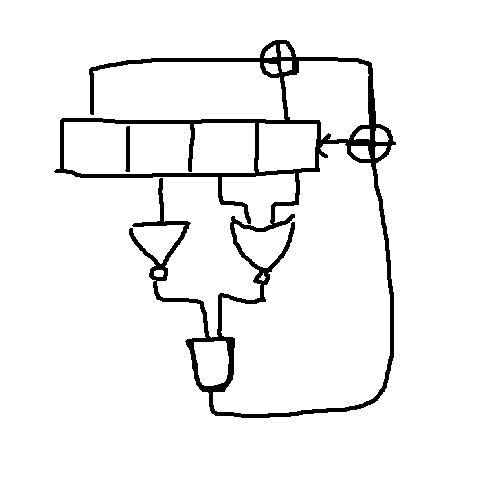
\includegraphics[scale=0.8]{gates.png}

\section{Laboratory exercise 5}
Let $f: \mathbb{Z}_2^4 \times \mathbb{Z}_5^4 \rightarrow \mathbb{Z}_{10}^4$ be defined as $$f(x, y) = 625x + y,$$
where $x\in [0, 15]$ and $y\in [0, 624]$. Then, $f$ is a bijective function.

\begin{proof}
Let $y$ be fixed, then
\begin{align*}
f(x_1, y) &= f(x_2, y) \\
625x_1 + y &= 625x_2 + y \\
625x_1 &= 625x_2 \\
x_1 &= x_2
\end{align*}
Let $x$ be fixed, then
\begin{align*}
f(x, y_1) &= f(x, y_2) \\
625x + y_1 &= 625x + y_2 \\
y_1 &= y_2
\end{align*}
Thus, the function $f$ is injective.

Let $z = [0, 9999] \subset \mathbb{Z}$.
Then, $$z = z_1 \cup \cdots \cup z_{15},$$ where $z_i = [625i, 625i + 624]$ and $0 \leq i \leq 15$. Clearly, the intervals $z_i$ are all disjoint.

Let $z^* \in z_1 \cup \cdots \cup z_{15}$. Then, $z^*$ can only be in one sub-interval $z_i$ of $z$, as all sub-intervals are disjoint, and $z^*$ can then be written as $z^* = 625i + c$ where $c \in [0, 624]$ and $i\in [0, 15]$.

Thus, picking $y = c$ and $x = i$ gives us a solution, and the function is then surjective.
\end{proof}

Let $f: \mathbb{Z}_2 \times \mathbb{Z}_5 \rightarrow \mathbb{Z}_{10}$. Then, defining $f(x, y) = 5x + y$ creates a bijective function.

\begin{verbatim}
package main

import (
  "fmt"
  "io"
  "os"
  "strings"
)

func WriteStringToFile(filepath, s string) error {
  fo, err := os.Create(filepath)
  if err != nil {
    return err
  }
  defer fo.Close()

  _, err = io.Copy(fo, strings.NewReader(s))
  if err != nil {
    return err
  }

  return nil
}

func mod(a int, n int) int {
  if a % n < 0 {
    return (a % n) + n
  } else {
    return a % n
  }
}


// Non-linear FSRs with 0-state
func LFSR2(poly []int, state[]int, n int) (out int, in int) {
  for i := 0; i < len(poly); i++ {
    in = in - poly[i] * state[i]
  }

  if (state[0] != 0 &&
    state[1] == 0 &&
    state[2] == 0 &&
    state[3] == 0) {
    return 1, 0
  } else if (state[1] == 0 &&
    state[2] == 0 &&
    state[3] == 0) {
    return 0, 1
  } else {
    return state[0], mod(in, n)
  }
}

func LFSR5(poly []int, state[]int, n int) (out int, in int) {
  for i := 0; i < len(poly); i++ {
    in = in - poly[i] * state[i]
  }

  if (
    state[0] == 2 &&
    state[1] == 0 &&
    state[2] == 0 &&
    state[3] == 0) {
    return 2, 0
  } else if (
    state[0] == 0 &&
    state[1] == 0 &&
    state[2] == 0 &&
    state[3] == 0) {
    return 0, 1
  } else {
    return state[0], mod(in, n)
  }
}

// Bijective function phi: Z_2 x Z_5 -> Z_10
func phi(x int, y int) int {
  return 5 * x + y
}

func main() {
  p := []int{1, 0, 0, 1}
  q := []int{2, 2, 1, 0}
  state2 := []int{0, 0, 0, 0}
  state5 := []int{0, 0, 0, 0}
  seq := make([]int, 0)

  for i := 0; i < 10003; i++ {
    out2, in2 := LFSR2(p, state2, 2)
    out5, in5 := LFSR5(q, state5, 5)

    state2 = append(state2[1:], in2)
    state5 = append(state5[1:], in5)

    seq = append(seq, phi(out2, out5))
  }

  if err := WriteStringToFile("input", strings.Trim(strings.Join(strings.Fields(fmt.Sprint(seq)), ""), "[]")); err != nil {
    panic(err)
  }
}
\end{verbatim}

% \begin{thebibliography}{9}
% \bibitem{prime} 
% Prime Counting function, \\
% \texttt{http://mathworld.wolfram.com/PrimeCountingFunction.html}
% \end{thebibliography}

\end{document}
